
\section{Digital Signals}
Complex exponential sequence: \(x(n) = Ae^{j(\omega_0n+\varphi)} = A \cos(\omega_0n+\varphi) + jA\sin(\omega_0n+\varphi)\),
with \(\omega_0=\frac{2\pi}{T_0}=2\pi f_0 = 2 \pi \frac{f}{f_s}\)

\textbf{Discrete Fourier Series}: \(\displaystyle \ x(n)=\frac{1}{N}\sum_{k=0}^{N-1}X(k)e^{j\overbrace{(2\pi/N)k}^{\omega_0(k)}n}
\ \Leftrightarrow \ X(k)=\sum_{k=0}^{N-1}x(n)e^{-j(2\pi/N)kn} = \textstyle X(f{=}\frac{f_s k}{N})
\quad( 0 \le k,n < N)\)

\begin{minipage}[t]{0.49\textwidth}
    \textbf{DFT properties}\\
    \begin{tabular}{@{}lll@{}}\toprule
        Property & Time Domain & Frequency Domain \\ \midrule
        Periodicity & \(x(n) = x(n+N)\) & \(X(k) = X((k))_N\) \\
        Linearity & \(ax_1(n) + bx_2(n)\) & \(aX_1(k) + bX_2(k)\) \\
        Convolution & \(x_1(n) * x_2(n)\) & \(X_1(k) X_2(k)\) \\
        Multiplication & \(x_1(n) x_2(n)\) & \(\frac{1}{N}(X_1(k) * X_2(k))\) \\
        \bottomrule
    \end{tabular}
\end{minipage}
\hfill
\begin{minipage}[t]{0.49\textwidth}
    \textbf{LTI systems}\\
    Output: \(y(n) = \sum_{k=-\infty}^{\infty}x(n)h(n-k) = x(n) * h(n)\)\\
    Frequency response \(H(\omega)\): \(Y(\omega)=X(\omega)H(\omega)\)\\
    FIR Filter: \(y(n)=a_0x(n) + a_1x(n-1) + \cdots + a_px(n-p)\)
\end{minipage}


\section{Speech Signals}
\textbf{Information content}: What?, Who?, How?, speaking environment, transmission channel, background noise

\textbf{Phonemes}: Smallest sound unit, speaker-independent. Western languages have 20 to 60 phonemes (German: 48).\\
\textbf{Phones}: Acoustic representation of the phoneme, speaker-dependent.

\textbf{Short-time spectral analysis}: Calculate the spectrum of a sliding window.
Idea: speech signal is quasi-stationary inside the window.
Spectrum of the windowed signal: \(\bar{X}(\omega)=X(\omega)*W(\omega)\).
Smoother window \(\leftrightarrow\) lower side lobes. Longer window \(\leftrightarrow\) higher spectral resolution.
The \textbf{Spectrogram} shows the temporal changes in the signal spectrum.

\textbf{Formants} are high energy areas in the spectrogram (usually dark).
The fundamental frequency \(F_0\) ranges from 50~Hz (deep mans voice) to 400~Hz (child), depending on the speaker.
The formants \(F_1\) to \(F_4\) convey information about the phone sequence.
\(F_1\) and \(F_2\) are speaker dependent.

\begin{minipage}[t]{0.35\textwidth}
\centering
\textbf{Vowels}
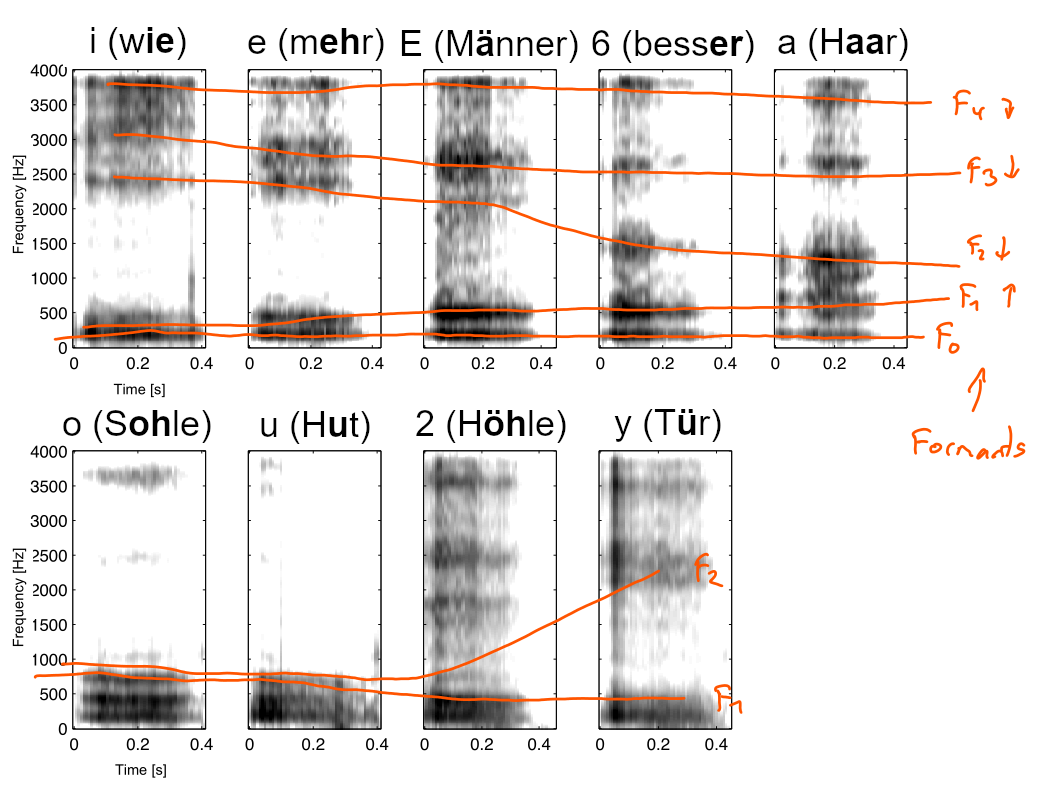
\includegraphics[width=\textwidth]{img/vowels}
\textbf{Diphthongs}
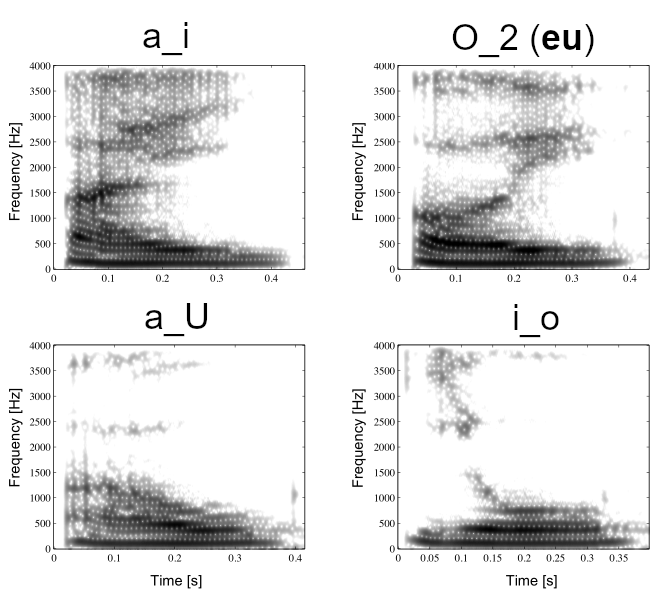
\includegraphics[width=0.9\textwidth]{img/diphthongs}
\end{minipage}
\hfill
\begin{minipage}[t]{0.31\textwidth}
\centering
\textbf{Fricatives (unvoiced)}
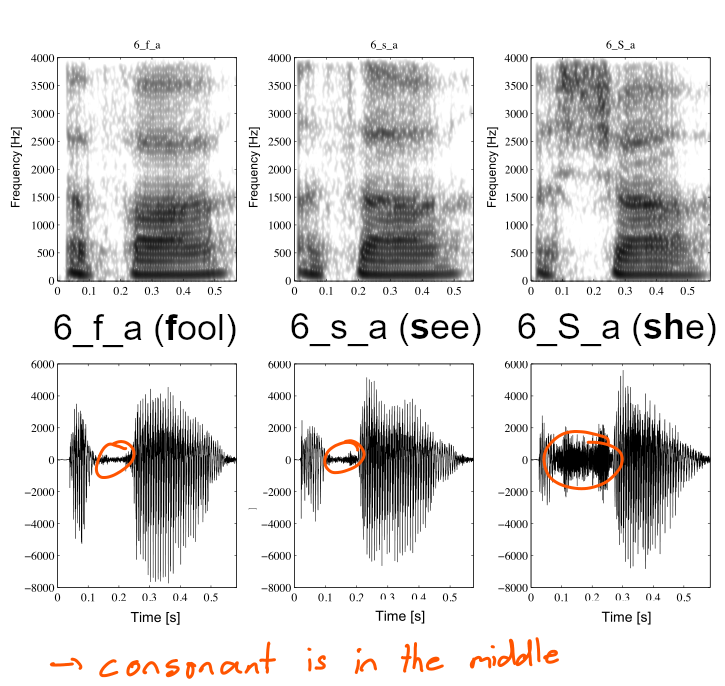
\includegraphics[width=\textwidth, trim={0 0 0 3mm}, clip]{img/fricatives_unvoiced}
\textbf{Nasals / Laterals}
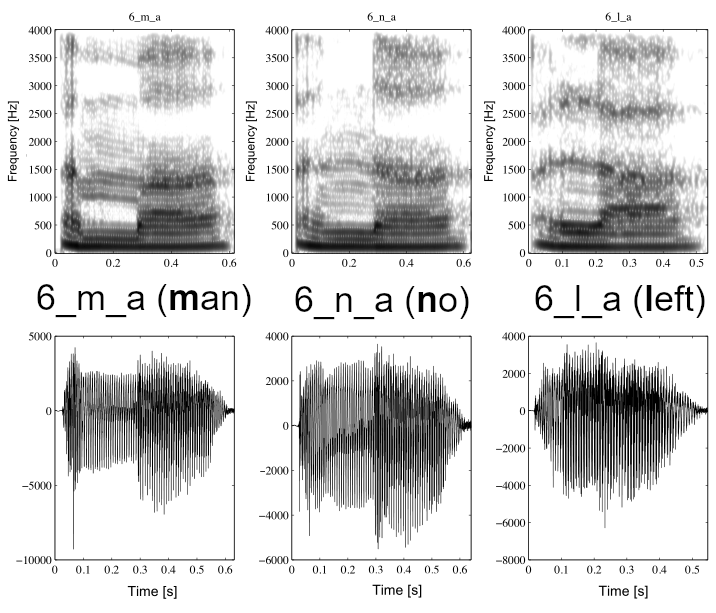
\includegraphics[width=\textwidth]{img/nasals_laterals}
\end{minipage}
\hfill
\begin{minipage}[t]{0.32\textwidth}
\centering
\textbf{Plosives (voiced)}
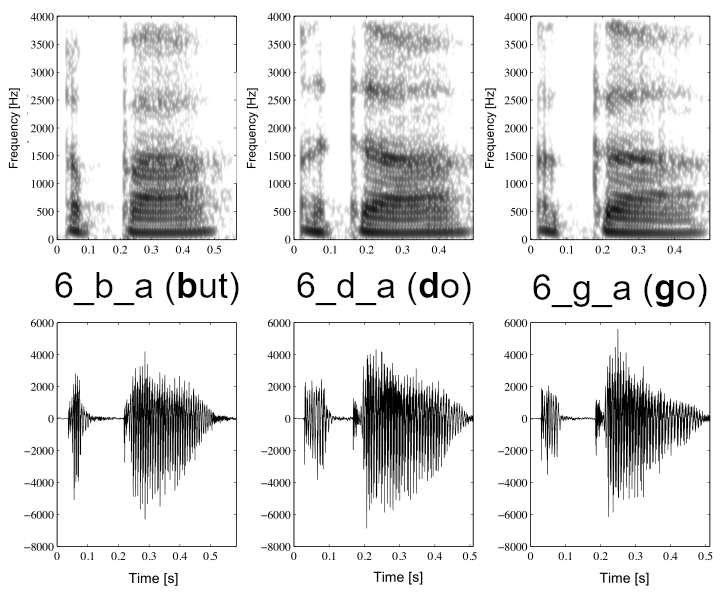
\includegraphics[width=\textwidth]{img/plosives_voiced}
\textbf{Plosives (unvoiced)}
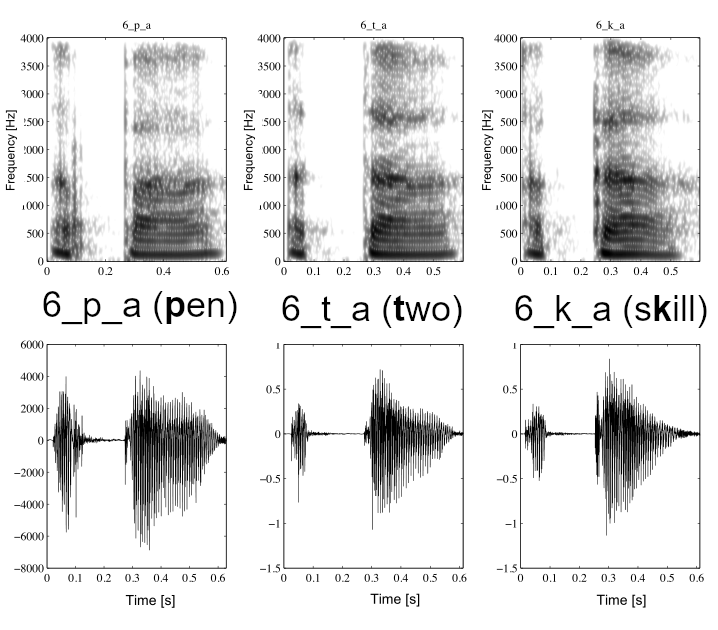
\includegraphics[width=\textwidth]{img/plosives_unvoiced.png}
\end{minipage}


\begin{minipage}[]{0.49\textwidth}
\centering
\textbf{Utterance of ``Sieben''} with \(F_0=100\)~Hz (male)
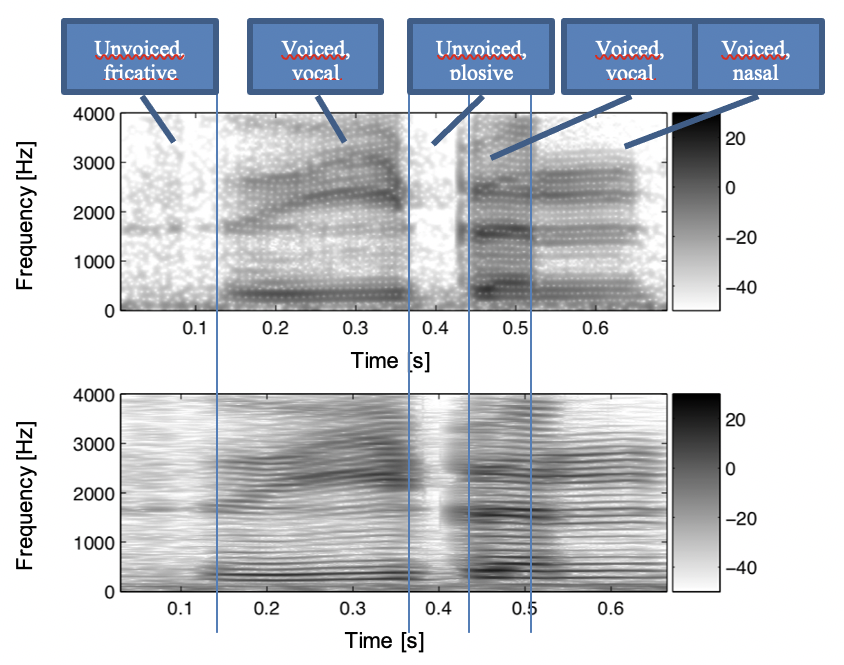
\includegraphics[width=\linewidth]{img/spectrogram_sieben}
\end{minipage}
\hfill
\begin{minipage}[]{0.4\textwidth}
\centering
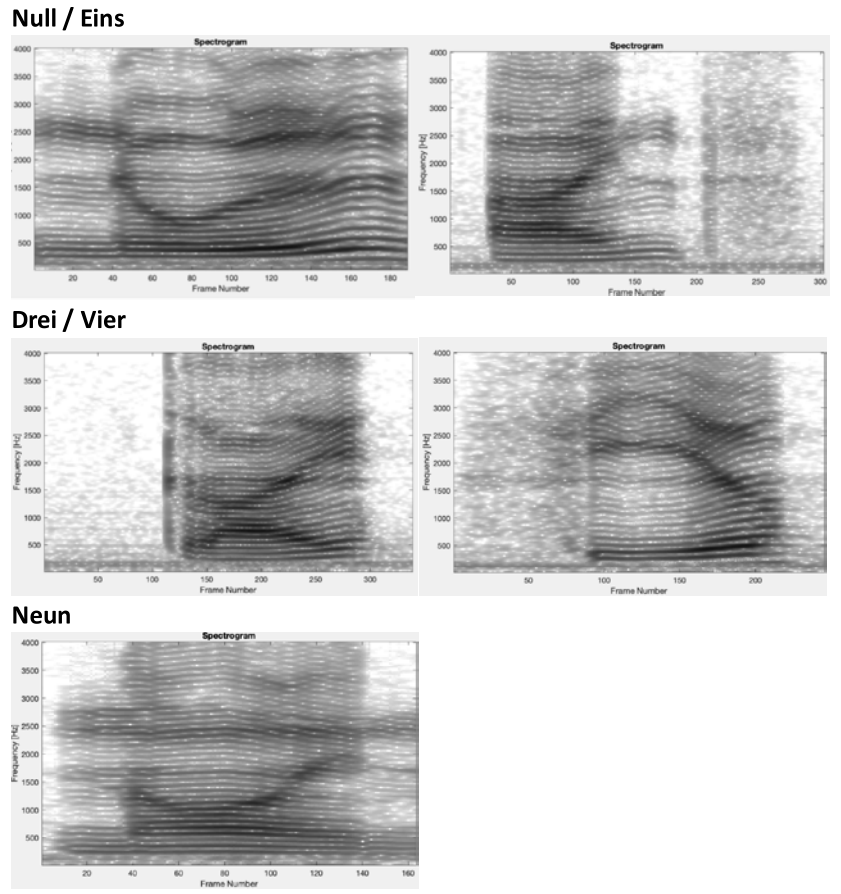
\includegraphics[width=\linewidth]{img/german_digits}
\end{minipage}


\subsection{Speech Recognition}
Speech recognition is the technology that converts spoken language into written text,
allowing computers to understand and process verbal commands or transcribe spoken words.
Very difficult because human voices can be very different, humans make mistakes, background noises and different acoustics for different environments.
Also, there are no word boundaries in human speech.

\subsubsection{Feature Extraction}
For speech recognition, spectrograms and the formants are important features.
Unimportant information can be filtered out by many means,
e.g. DFT-Cepstrum (IDFT of the Log of the DFT-Spectrum) to extract the source (vocal excitation) from the filter (vocal tract) components.
A Mel-Spectrum is a spectrum that more closely resembles the characteristics of the human ear by having logarithmic sensitivity
for frequencies above 1~kHz (lower sensitivity for higher frequencies).
Mel-Cepstrum: IDFT of Log(Mel-Spectrum). The Fast Cochlea Transform (FCT) is a signal processing technique inspired by the auditory processing in the human cochlea.

\subsubsection{Classical Approaches: Rule- based and Pattern Matching}
Both require feature extraction from the speech signal.

Rule- based: Classification is based on rules for each class derived from human knowledge/observation.
Very difficult because not generalizable for different speakers.

Pattern Matching: Classification based on a distortion measure between a feature pattern and given reference patterns for each class (kNN, SVMs).
Main problem is that the patterns can also vary in the temporal structure.
We can use Dynamic Time Warping (DTW) to align the extracted features to the reference features by
locally stretching or squeezing pattern by duplicating or dropping feature vectors.

\subsubsection{Statistical Classification}
To calculate joined probabilities, we can use bayes rule: $ P(X | W) = \frac{P(W | X) \cdot P(W)}{P(X)} $

Given extracted feature  $ X $ from the speech recognizer, the MAP classifier must choose the word sequence $ W $
that has the highest a-posteriori probability of all possible word sequences.

\subsubsection{Hidden Markov Model (HMM)}
Defined by N states, state transition probabilities as well observation probability distribution in each emitting state.

Forward Algorithm: Given a HMM $ \lambda $, a sequence of emitted observations $ \textbf{X} = x_1, x_2, \ldots, x_T $,
we want to efficiently calculate $ P(\textbf{X} | \lambda) $. Known as Evaluation problem.
Brute force approach would be to simply try out all state combinations and see which one has the highest likelihood of giving the seen sequence.
Forward algorithm takes advantage of independent states and instead keeps the probabilities for emitting the observations for each state. Forward: Addition.

Viterbi Algorithm: Given a HMM $ \lambda $, a sequence of emitted observations $ \textbf{X} = x_1, x_2, \ldots, x_T $,
we want to efficiently calculate the most likely state sequence $ Q* = \max_Q P(Q | \textbf{X}, \lambda) $.
Known as Decoding Problem. Same idea as Forward, but instead of adding all possibilities, we always take the max.
N-best Viterbi outputs the N-best state sequences instead of only the best.

Forward-Backward algorithm/Baum-Welch algorithm: Given a sequence of emitted observations $ \textbf{X} = x_1, x_2, \ldots, x_T $ and a model structure,
find parameters for HMM $ \omega $ such that $ \omega* = \max_{\lambda} P(\textbf{X} | \lambda) $.
Known as Estimation Problem. How HMMs are trained.
Forward-Backward estimates the probabilities of the sequence given the current models while Baum-Welch applies changes to optimize the parameters,
kind of like backpropagation.

\subsubsection{HMM Speech Recognizer}
Speech recognition is done with HMMs of sub-units that are concatenated to word and sentence recognition networks.
Viterbi then finds the most likely path through the network.
State sequence $ \xrightarrow{} $ subunit sequence $ \xrightarrow{} $ word sequence $ \xrightarrow{} $ sentence

Lexicon: Describes pronounciation of all words allowed; Language model: Describes all utterances allowed and their probabilities.
Typically, Mel-Cepstrum, Delta-Cepstrum or other are used as features.

Disadvantages: HMM assumptions never totally met in practice: Conditional independence of states and observations;
Training HMMs is not inherently discriminative but rather likelihood maximizing.

\subsubsection{Deep Learning Speech Recognizer}
\textbf{Datasets}: Split dataset into training and test/evaluation sets.
\textbf{Word Error Rate}: Count substitutions (S), insertions (I), deletions (D) and divide by number of words in ground truth.
\textbf{Data Preprocessing} Scale input data to have zero mean and unit variance.
\textbf{Initialization}: use random gaussian distributed weights.
\textbf{Overfitting}: Memorizing the training set. Use dropout to mitigate.
\textbf{Batch Size}: Compromise between faster and more optimal training.
\textbf{Batch Normalization}: Scale the activations to have zero mean and unit variance (only during training).

Normal Depp Neural Networks (DNN) classify only input patterns of constant size (e.g. image), so other architectures are used.

\textbf{DNN-HMM}: Use DNN as feature extractor for HMM; \textbf{CNN}: Use CNN on spectrogram;
\textbf{LSTM vs. GRU}: both types of recurrent neural network (RNN) architectures designed to address the vanishing gradient problem in traditional RNNs.
LSTMs have a more complex memory cell that consists of a cell state and three gates - input gate, forget gate, and output gate.
GRUs have a simpler memory cell with two gates - reset gate and update gate.
